\documentclass{article}
\usepackage[utf8]{inputenc}
\usepackage{graphicx}
\graphicspath{.}
\usepackage{amsmath}
\usepackage{hyperref}
\usepackage{amssymb}
\usepackage{xcolor}
\title{ECE310 Final Review - Cramming Carnival}
\author{Author: Members of HKN}
\date{Fall 2024}
\newcommand{\dd}[1]{\mathrm{d}#1}

\usepackage[makeroom]{cancel}
\usepackage[letterpaper, portrait, margin=1in]{geometry}
    
\pagenumbering{arabic}

\begin{document}

\maketitle

\section{Questions}
Note: Unless stated otherwise, assume all *sequences* of form $f[n]$ are \textit{real valued}.

Note 2: Content for this class varies semester by semester. If you see something that you know will not be on the exam, you can ignore it.
\subsection{Sacrilegious Sampling}
\subsubsection{Frugal Sampling}
You are working on a system with Dr. Dee Efty that takes an analog signal as input, converts it to digital, filters the digital signal, and converts it back to analog. He tells you that the input analog signal is bandlimited at 60kHz, but nothing else. A bad sampling rate is an issue for everybody - you'll need more memory to store the larger number of samples, and the hardware to sample faster will undoubtedly cost more. So, you ask Dr. Efty via email what the filter will look like, and he has \textit{yet} to respond.

\begin{enumerate}
    \item Knowing nothing about the filter, what is the smallest sampling rate for the A/D converter that will result in LTI operation? \vspace{1.5cm}
    \item FINALLY, Dr. Efty gets back to you. Below are a set of possible responses from Dr. Efty. For each, report whether the minimum sampling rate for LTI operation can be made smaller, or whether the sampling rate remains the same.
    \begin{enumerate}
        \item "Oh, the filter we want to implement is a lowpass cutting off at 10kHz." \vspace{1.5cm}
        \item "The filter is a bandpass, permitting frequencies from 20kHz to 30kHz to pass through." \vspace{1.5cm}
        \item "The desired filter is a highpass with cutoff at 40kHz." \vspace{1.5cm}

    \end{enumerate}
\end{enumerate}

\newpage
\subsubsection{Up Up, Down Down, ...}
Suppose we are given the signal $x[n] \overset{DTFT}{\longleftrightarrow} X(\omega)$ below: \\
\begin{center}
    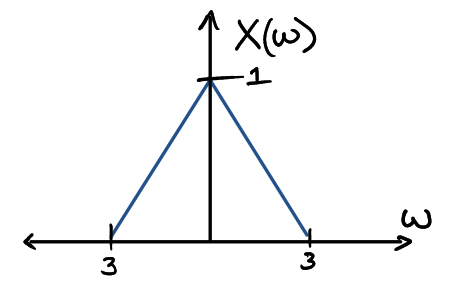
\includegraphics[scale=0.25]{figures/simple-signal-1.png}
\end{center}

\begin{enumerate}
    \item Let $x_u[n] \overset{DTFT}{\longleftrightarrow} X_u(\omega)$ be the result of upsampling $x[n]$ by a factor of 4. Sketch $X_u(\omega)$ below. \vspace{2cm}
    \item Let $x'[n]$ be the result of passing $x_u[n]$ through a low pass filter with cutoff frequency $\omega_c=\frac{\pi}{2}$. Let $y[n] \overset{DTFT}{\longleftrightarrow} Y(\omega)$ be the result of downsampling $x'[n]$ by a factor of 2. Sketch $Y(\omega)$ below.\vspace{2cm} 
\end{enumerate}
\subsection{Freaky Filters}
\subsubsection{FIR, Step-by-Step}
Dr. Dee Efty is back with more tasks for you. You are asked to make an FIR filter $h[n]$ that implements $D(\omega)$, a desired frequency response, where on the interval $\omega \in [-\pi, \pi)$:
    \[
        D(\omega) = \begin{cases}
            1 & \vert \omega \vert < 0.5 \\
            0 & \text{else}
        \end{cases}
    \]

\begin{enumerate}
    \item 
    Dr. Efty has employed the help of an ECE 408\footnote{The entire latter half of the class is about implementing block convolution on NVIDIA GPUs. Not even joking.} student to write FIR convolution code on a GPU. The student successfully wrote their code, but due to off-by-one errors, it only works on filters with \textit{even} length. Furthermore, due to the limitations of the hardware, the filter can have at most $64$ values.
    \begin{enumerate}
        \item Is it possible to make this filter, and if so, what is the maximum length of the FIR filter for which the filter is possible?
        \item Circle the correct choices: The filter as described above must have \textbf{odd}/\textbf{even} symmetry, and the type must be \textbf{type I}/\textbf{type II}/\textbf{type III}/\textbf{type IV} for the filter with maximal length. 
    \end{enumerate}
    \item
    You report your results to Dr. Efty, and he decides last minute to change the filter specification to a highpass with cutoff $\omega_c = \frac{1}{2}$, and to implement the filter with \textbf{odd} symmetry and \textbf{even} length $L=8$. That is to say, the desired frequency response on the interval $\omega \in [-\pi, \pi)$ is:
    \[
        D(\omega) = \begin{cases}
          0 & \vert \omega \vert < 0.5 \\
          1 & \text{else}
        \end{cases}
    \]
    \begin{enumerate}
        \item Circle the correct choice: this new filter is now a \textbf{type I}/\textbf{type II}/\textbf{type III}/\textbf{type IV} filter.
        \item Let $H'(\omega)$ represent the DTFT of the above filter with the given specifications \textit{without} any delay or windowing applied. Sketch $|H'(\omega)|$ and $\angle H'(\omega)$. \vspace{2cm}
        \item What is the necessary time delay $d$ to apply to $H'(\omega)$?
        \item After adding this delay, what is the DTFT of the \textit{unwindowed} frequency response of the FIR filter, $H_{u}(\omega)$? Express it in terms of $H'(\omega)$, and then express it in terms of $D(\omega)$. \vspace{2cm}
        \item What is the expression for $h_u[n]$, the unwindowed filter? \vspace{2cm}
    \end{enumerate}
    \item Let $h'[n] \overset{DTFT}{\longleftrightarrow} H'(\omega)$ be the filter \textit{before} delaying and windowing, as from earlier. Let $h[n]$ be the final, \textit{windowed} and \textit{delayed} FIR filter. Assuming that the window used is \textbf{rectangular}, if $h[k]=h'[m]$, then write $k$ under the corresponding box for $h'[m]$. For example, if $h'[3]=h[4]$ but the value of $h'[3.5]$ is never used for $h[n]$, then only write "$4$":
    \begin{center}
        \begin{tabular}{|c|c|c|}
             \hline
             $n$ for $h'[n]$ & 3 & 3.5 \\
             \hline
             $n$ for $h[n]$ & \textbf{4} & (leave blank) \\
             \hline
        \end{tabular}
    \end{center}
\begin{center}
    \begin{tabular}{|c|c|c|c|c|c|c|c|c|}
         \hline
        $n$ for $h'[n]$ & -8.5 & -8 & -7.5 & -7 & -6.5 & -6 & -5.5 & -5 \\
        \hline
        $n$ for $h[n]$ &  &  &  &  &  & & &   \\
        \hline
        $n$ for $h'[n]$ & -4.5 & -4 & -3.5 & -3 & -2.5 & -2 & -1.5 & -1 \\
        \hline
        $n$ for $h[n]$ &  &  &  &  &  & & &   \\
        \hline
        $n$ for $h'[n]$ & -0.5 & 0 & 0.5 & 1 & 1.5 & 2 & 2.5 & 3 \\
        \hline
        $n$ for $h[n]$  &  &  &  &  &  & & &\\
        \hline
        $n$ for $h'[n]$ & 3.5 & 4 & 4.5 & 5 & 5.5 & 6 & 6.5 & 7 \\
        \hline
        $n$ for $h[n]$  &  &  &  &  &  & & &\\
        \hline
    \end{tabular}
\end{center}
\hspace{10mm}
    
\end{enumerate}

\newpage

\subsection{I Got 99 Block Diagrams, but...}
Suppose we are given the difference equation system $H$, described by: $$y[n] + 8y[n-1]+15y[n-2]=-x[n]+x[n-2]$$
\begin{enumerate}
    \item What is the z-transform, $H(z)$? Assume the system is causal. \vfill
    \item Draw below the block diagram in \textbf{direct form I}. \vfill
    \item Draw below the block diagram in \textbf{direct form II}.\vfill
    \item Draw below the block diagram in \textbf{direct form II, transposed}. \vfill
    %\iffalse
    \item Draw below the block diagram in \textbf{cascade for direct form I}.\vfill
    \item Draw below the block diagram in \textbf{parallel for direct form I}.\vfill
    %\fi
\end{enumerate}
\newpage
\subsection{Delightful DFTs}
\subsubsection{Math Without Calculators}
Consider the two below sequences:
\[
\left\{x[n]\right\}_{n=0}^{3} = \left\{ 1, 2, 0, 2 \right\}, 
\left\{y[n]\right\}_{n=0}^{3} = \left\{ 3, 1, -1, 1 \right\}
\]
\begin{enumerate}
    \item Calculate the 4-point DFT of $x[n]$, $X[k]$, using an FFT butterfly decimated in time. \vspace{4cm}
    \item Calculate the 4-point DFT of $y[n]$, $Y[k]$, using an FFT butterfly decimated in frequency.\footnote{Fun fact: applying the transposition operation that you know from block diagrams to the decimation-in-time butterfly, yields the decimation-in-frequency butterfly! Same with the other way around.} \vspace{4cm}
    \item Calculate $z[n] = x[n] \circledast y[n]$, the circular convolution of $x[n]$ and $y[n]$. \vspace{4cm}
    \item Calculate the 4-point DFT of $z[n]$, $Z[k]$, using whatever method you would like. \\ 
    Verify that $Z[k_i]=Y[k_i]X[k_i]$ for $i \in \{0, 1, 2, 3\}$.
    \vspace{4cm}

\end{enumerate}

\subsection{Famous FFTs}

After a wonderful dinner with Dr. Efty, where the two of you discussed important applications of the FFT, you retire back to your room with an important napkin. On the napkin is a beautiful diagram that Dr. Efty had given to you as a proof for a most illuminating theorem. Unfortunately, during the scramble to figure out who was going to pay, some Sprite got on the napkin. Below is remainder of the diagram.

You recall that the diagram was once part of a 64-bit decimation in time radix-2 FFT. You must find the values of the red letters and greek letters so that you can publish another paper.

\begin{figure}[h]
\begin{center}
    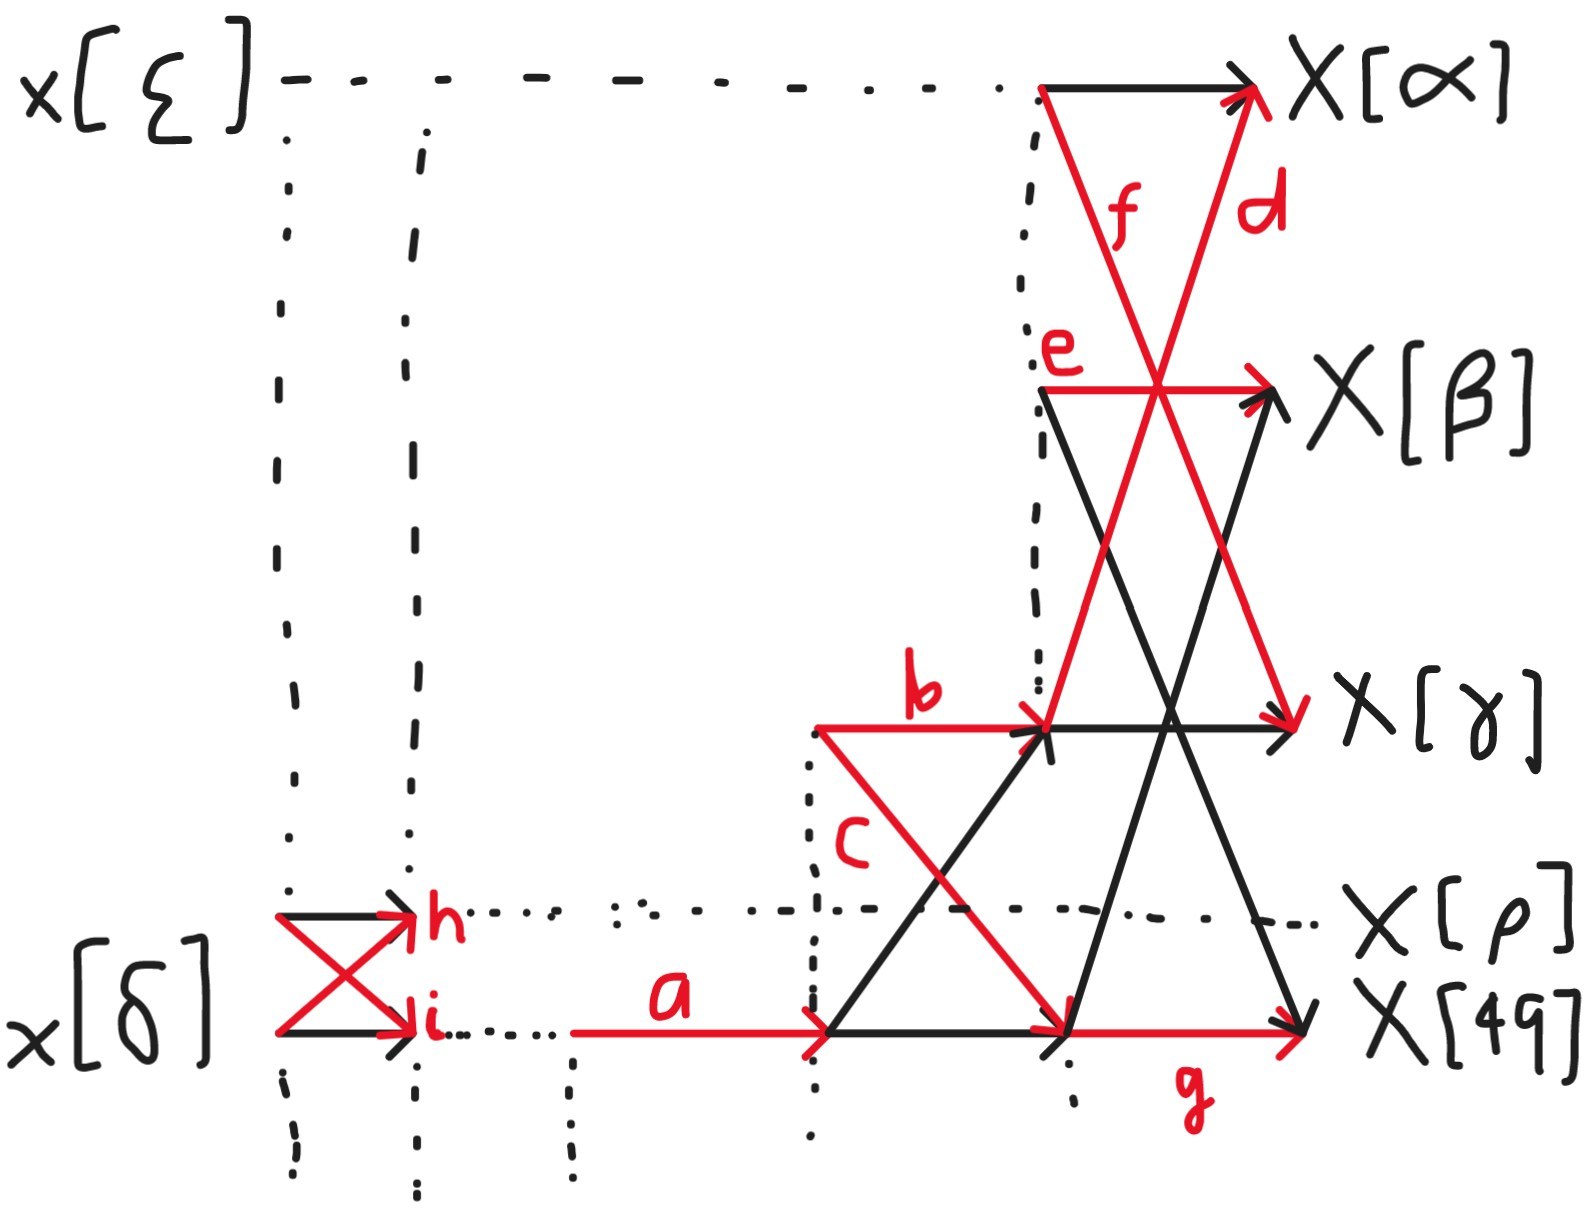
\includegraphics[width=0.8 \textwidth]{figures/FFT Diagram.jpg}
    \caption{The Remains of the Napkin}
    \label{fig:FFT_diagram}
\end{center}
\end{figure}

\newpage

\subsection{Lethargic Linear Algebra}

Later in the night, you and Dr. Efty engage in a bit of merriment, and Dr. Efty's memory starts to get a little fuzzy. Dr. Efty wants to develop an adaptive filter to fix his noisy radio, as his favorite songs are now distorted, which is ruining his mood. To do this, he knows he will need some linear algebra, but is having some trouble remembering concepts. It is up to you to help him.

\begin{enumerate}
    \item Firstly, he remembers that he will need to solve an optimization problem, namely that of:
    $$\boldsymbol{w^*} = \underset{\boldsymbol{w}}{\arg\min} ||\boldsymbol{X^\top w} - \boldsymbol{t}||^2$$
    He vaguely remembers that the optimal solution to this problem is given as :
    $$\boldsymbol{w^*} = (\boldsymbol{XX^\top})^{-1}\boldsymbol{Xt}$$
    He would like you to prove that this is the case (Hint: use gradients).
    \vspace{4cm}
    \item Dr. Efty would now like you to create an ideal filter satisfying this constraint. He plays you the tune coming out of his radio, and it goes like this:
    $$\left\{x[n]\right\}_{n=0}^{1} = \left\{ 1, 2 \right\}$$
    He listens to rather simple music. He knows that this is a noisy signal, and hums you what the song should sound like, and hums a slightly longer section of the song. It goes like so:
    $$\left\{t[n]\right\}_{n=0}^{2} = \left\{ 2, 7, 6 \right\}$$
    Given this information, construct a length-2 filter $\boldsymbol{w}[n]$ that performs optimal filtering, using the equation derived in the previous question.
    \newpage
    \item Dr. Efty knows that using the DFT will help him analyze the filter, or something. To practice, this he looks at a filter given by:
    $$\left\{h[n]\right\}_{n=0}^{3} = \left\{ 1, 2, 0, 2 \right\}$$
    (This is the same as the signal from problem 1.4) He would like you to take the normalized DFT by writing out and performing the matrix multiplication, $\boldsymbol{F^*h}$.
    
    \vspace{10cm}
    \item Dr. Efty now wants you to prove that the basis vectors of the Fourier transform matrix $\boldsymbol{F^*}$ form an orthonormal basis (Hint: the row vectors happen to form the basis vectors). For the sake of this problem, it is fine merely to show that the matrix $\boldsymbol{F^*}$ from the last problem is orthonormal.
\end{enumerate}

\end{document}